% !TEX program = xelatex
% !TEX encoding = UTF-8
% !BIB program = bibtex
% !TEX spellcheck = en_US
\documentclass[12pt]{article}
\usepackage[letterpaper, margin=1in]{geometry}
\usepackage{amsmath,amssymb}
\usepackage{graphicx}
\usepackage{subfigure}
\usepackage{newpxtext,newpxmath}
\usepackage{siunitx}
\usepackage{hyperref}
\usepackage{bm}
\usepackage[version=4]{mhchem}
\usepackage{tikz}
\usetikzlibrary{calc}
\usetikzlibrary{arrows.meta}
\usetikzlibrary{decorations.pathreplacing}
\usetikzlibrary{decorations.pathmorphing}
\usepackage{relsize}
\tikzset{fontscale/.style = {font=\relscale{#1}}
}
\usepackage{wrapfig}
\usepackage{lipsum}

\makeatletter
\newcommand{\gettikzxy}[3]{%
  \tikz@scan@one@point\pgfutil@firstofone#1\relax
  \edef#2{\the\pgf@x}%
  \edef#3{\the\pgf@y}%
}
\makeatother

\title{Spinodal Decomposition}
\author{}
\date{}

\begin{document}
\maketitle

Consider a binary alloy system with a miscibility gap,
i.e.,
\begin{figure}[h]
	\begin{minipage}[l]{0.3\textwidth}
		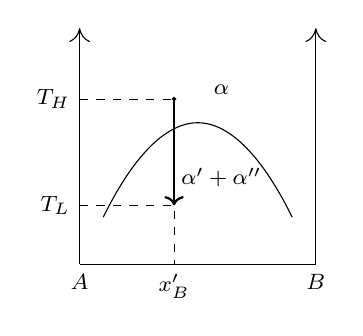
\begin{tikzpicture}[scale=3, font=\footnotesize]
	% axis
	\draw [-{>[scale=2.5,
    length=2,
    width=3]}] (0,0) -- (0,1);
	\draw (0,0) -- (1,0);
	\draw [-{>[scale=2.5,
    length=2,
    width=3]}] (1,0) -- (1,1);

	% curve
	\coordinate (A) at (0.1,0.2);
	\coordinate (B) at (0.9,0.2);
	\draw (A) parabola[bend pos=0.5] bend +(0,0.4) (B);

	% line
	\coordinate (xb') at (0.4,0);
	\coordinate (TL) at (0,0.25);
	\coordinate (TH) at (0, 0.7);
	\draw[dashed] (TL) -| (xb');
	\draw[dashed] (TH) -- ($ (xb') + (TH) $);

	% arrow
	\draw[->, thick] ($ (xb') + (TH) $) -- ($ (xb') + (TL) $);

	% point
	\draw[fill=black] ($ (xb') + (TH) $) circle[radius=0.2pt];

	% text
	\draw (TH) node[anchor=east] {$T_H$};
	\draw (TL) node[anchor=east] {$T_L$};
	\draw (0.6,0.45) node[anchor=north] {$\alpha'+\alpha''$};
	\draw (0.6,0.8) node[anchor=north] {$\alpha$};
	\draw (xb') node[anchor=north] {$x_B'$};
	\draw (0,0) node[anchor=north] {$A$};
	\draw (1,0) node[anchor=north] {$B$};
\end{tikzpicture}
	\end{minipage}%
	\hfil
	\begin{minipage}[r]{0.6\textwidth}
		now, consider a transformation which must occur when an alloy
		with composition $x_B'$ is quenched from temperature $T_H$
		to a lower temperature $T_L$', i.e.,
		\begin{equation*}
			\ce{$\alpha$ -> $\alpha' + \alpha''$}.
		\end{equation*}
	\end{minipage}
\end{figure}

In order to properly deal with the transformation, we need to analyze,
not surprisingly, the $G_{\text{sol}}$ vs composition relation at the
transformation temperature $T_L$!

I.e.,
\begin{figure}[h]
	\begin{minipage}[l]{0.3\textwidth}
		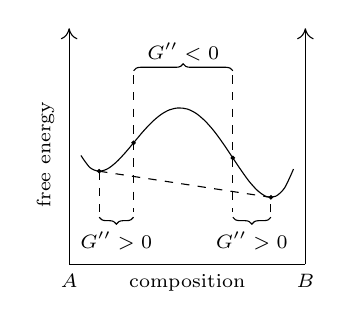
\begin{tikzpicture}[scale=3, domain=0.05:0.95, font=\scriptsize]
	% axis
	\draw [-{>[scale=2,
			length=2,
			width=3]}] (0,0) -- (0,1);
	\draw (0,0) -- (1,0);
	\draw [-{>[scale=2,
			length=2,
			width=3]}] (1,0) -- (1,1);

	\begin{scope}[yscale=0.5, yshift=0.5cm]
		% curve
		\coordinate (g00A) at (0.272815, 0.529808);
		\coordinate (g00B) at (0.692895, 0.402102);
		\coordinate (g0A) at (0.127138, 0.289339);
		\coordinate (g0B) at (0.854233, 0.0681958);
		\draw plot[smooth] (\x, {0.7 - 7.45598 * \x + 41.666 * \x^2 - 70.9531 * \x^3 + 36.7362 * \x^4});
	\end{scope}


	% line
	\gettikzxy{(g00A)}{\ax}{\ay};
	\gettikzxy{(g00B)}{\bx}{\by};
	\gettikzxy{(g0A)}{\fax}{\fay};
	\gettikzxy{(g0B)}{\fbx}{\fby};
	\draw[dashed] (\ax, 0.8) -- (\ax, 0.22);
	\draw[dashed] (\bx, 0.8) -- (\bx, 0.22);
	\draw[dashed] (g0A) -- (g0B);
	\draw[dashed] (\fax, \fay) -- (\fax, 0.22);
	\draw[dashed] (\fbx, 0.22) -- (\fbx, \fby);

	% point
	\draw[fill=black] (g00A) circle[radius=0.2pt];
	\draw[fill=black] (g00B) circle[radius=0.2pt];
	\draw[fill=black] (g0A) circle[radius=0.2pt];
	\draw[fill=black] (g0B) circle[radius=0.2pt];

	% text
	\draw (0.5, 0) node[anchor=north] {composition};
	\draw (0,0) node[anchor=north] {$A$};
	\draw (1,0) node[anchor=north] {$B$};
	\draw (-0.1,0.2) node[anchor=west, rotate=90] {free energy};
	\draw ($ ( {(\ax + \bx)/2}, 0.9) $) node (g) {$G'' < 0$};  % You need to wrap the expression into { } to hide the second pair of ( ) from the TeX parser.
	\draw ($ ( {(\fax + \ax)/2}, 0.1) $) node (g) {$G'' > 0$};
	\draw ($ ( {(\fbx + \bx)/2}, 0.1) $) node (g) {$G'' > 0$};

	% others
	\draw [
		decoration={
				brace
			},
		decorate
	] (\ax,0.82) -- (\bx,0.82);
	\draw [
		decoration={
				brace,
				mirror,
			},
		decorate
	] (\fax, 0.2) -- (\ax, 0.2);
	\draw [
		decoration={
				brace,
			},
		decorate
	] (\fbx, 0.2) -- (\bx, 0.2);
\end{tikzpicture}
	\end{minipage}%
	\hfil
	\begin{minipage}[r]{0.6\textwidth}
		In particular,
		\begin{enumerate}
			\item If $x_B'$ inside the $G''<0$ region, then small fluctuations
			      in composition $\Rightarrow G \downarrow$ about $x_B'$.
			      $\therefore$ system is unstable and decomposition continues via
			      ``uphill'' diffusion!
		\end{enumerate}
	\end{minipage}
\end{figure}

On the other hand,
\begin{enumerate}
	\setcounter{enumi}{1}
	\item If $x_B'$ outside the $G''<0$ region,
	      small variations in composition $\Rightarrow$ increase in the total
	      free energy of the system (i.e., $G \uparrow$).
	      $\therefore$ system is metastable and requires large fluctuations to
	      develop \ce{$\alpha' + \alpha''$} (i.e., N and G required here).
\end{enumerate}

Expand $G(c)$ about $c_0$, then
\begin{align*}
	G(c_0 + \Delta c) & =
	G(c_0) + G'(c_0) \cdot \Delta c +
	G''(c_0) \cdot \frac{ (\Delta c)^2 }{ 2! }
	+ \cdots,\\
	G(c_0 - \Delta c) & =
	G(c_0) - G'(c_0) \cdot \Delta c +
	G''(c_0) \cdot \frac{ (\Delta c)^2 }{ 2! }
	+ \cdots.
\end{align*}
\begin{equation*}
	\therefore \Delta G = \frac{ G(c_0 + \Delta c) + G(c_0 - \Delta c) }{ 2 }
	- G(c_0) = \frac{ G''(c_0) (\Delta c)^2 }{ 2 },
\end{equation*}
which is to say that $\Delta G < 0$ if $G''(c_0) < 0$ and $\Delta G > 0$ if
$G''(c_0) > 0$.

If we plot $G'' = 0$ points at various temperature, we obtain the chemical
spinodal (i.e., line of $G'' = 0$).

\begin{figure}[h]
  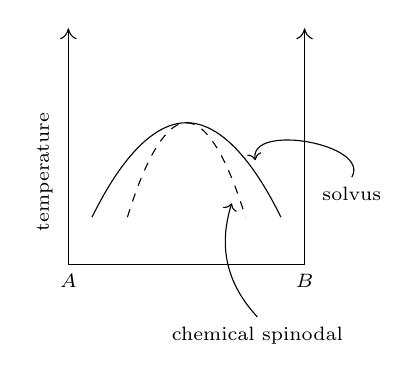
\begin{tikzpicture}[scale=3, font=\scriptsize]
	% axis
	\draw [-{>[scale=2,
			length=2,
			width=3]}] (0,0) -- (0,1);
	\draw (0,0) -- (1,0);
	\draw [-{>[scale=2,
			length=2,
			width=3]}] (1,0) -- (1,1);

	% curve
	\coordinate (A) at (0.1,0.2);
	\coordinate (B) at (0.9,0.2);
	\coordinate (C) at (0.25,0.2);
	\coordinate (D) at (0.75,0.2);
	\draw (A) parabola[bend pos=0.5] bend +(0,0.4) (B);
	\draw[dashed] (C) parabola[bend pos=0.5] bend +(0,0.4) (D);

	% node
	\draw (0,0) node[anchor=north] {$A$};
	\draw (1,0) node[anchor=north] {$B$};
	\draw (-0.1,0.1) node[anchor=west, rotate=90] {temperature};
	\draw (0.8, -0.3) node (n1) {chemical spinodal};
	\draw (1.2, 0.3) node (n2) {solvus};
	\draw (0.65, 0.3) node (ns1) {}; % chemical spinodal
	\draw (0.75, 0.4) node (ns2) {}; % solvus

	% reference
	\path[->] (n1.north) edge [out=180, in=0, bend left] (ns1.south east);
	\path[->] (n2.north) edge [out=60, in=100] (ns2.north east);
\end{tikzpicture}
\end{figure}

Inside the spinodal $\rightarrow$ spontaneous decomposition can occur
via ``uphill'' diffusion process, i.e.,

\begin{figure}[h]
	\centering
	\begin{minipage}[b]{.5\linewidth}
		\centering
		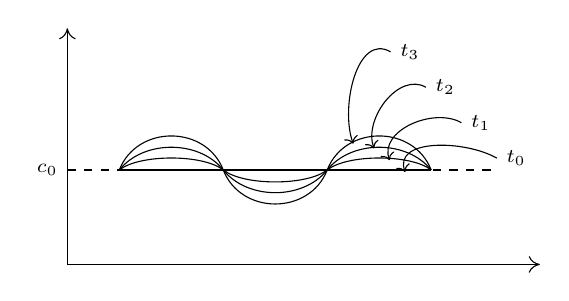
\begin{tikzpicture}[scale=3, font=\scriptsize]
	% axis
	\draw [-{>[scale=2,
			length=2,
			width=3]}] (0,0) -- (0,1);
	\draw[-{>[scale=2,
			length=2,
			width=3]}] (0,0) -- (2,0);

	% curve
	\begin{scope}[xscale=2.2, yshift=-0.1cm]
		\foreach \theta / \l in {0/0, 60/1, 70/1.75, 80/2.5}
		\draw (0.1,0.5) to [out=\theta, in=180-\theta, looseness=\l] (0.3,0.5)
		to [out=-\theta, in=\theta-180, looseness=\l] (0.5,0.5)
		to [out=\theta, in=180-\theta, looseness=\l] (0.7,0.5);
	\end{scope}

	\begin{scope}[yshift=-0.1cm]
  % line
  \draw[dashed] (0,0.5) -- (1.8,0.5);
  
  % node
  \draw (0,0.5) node[anchor=east] {$c_0$};
  \draw (2.2*0.65,0.45) node (c0) {};
  \draw (2.2*0.62,0.5) node (c1) {};
  \draw (2.2*0.59,0.55) node (c2) {};
  \draw (2.2*0.55,0.57) node (c3) {};
  \draw (1.9,0.55) node (t0) {$t_0$};
  \draw (1.75,0.7) node (t1) {$t_1$};
  \draw (1.6,0.85) node (t2) {$t_2$};
  \draw (1.45,1.0) node (t3) {$t_3$};
  
  % reference
  \path[->] (t0.west) edge [out=150, in=110] (c0.north);
  \path[->] (t1.west) edge [out=150, in=110] (c1.north);
  \path[->] (t2.west) edge [out=150, in=110] (c2.north);
  \path[->] (t3.west) edge [out=150, in=110] (c3.north);
  \end{scope}
\end{tikzpicture}
	\end{minipage}%
	\hfill
	\begin{minipage}[b]{.5\linewidth}
		\centering
		\begin{tikzpicture}[scale=3, font=\scriptsize, remember picture]
	% axis
	\draw [-{>[scale=2,
			length=2,
			width=3]}] (0,0) -- (0,1);
	\draw[-{>[scale=2,
			length=2,
			width=3]}] (0,0) -- (2,0);

	% line
	\begin{scope}[xscale=2.2, yshift=0.05cm]
		\draw (0.1,0.2) |- (0.3,0.5) |- (0.5,0.2) |- (0.7,0.5) -- (0.7,0.2);
		\draw[dashed] (0,0.2) -- (0.8,0.2);
		\draw[dashed] (0,0.5) -- (0.8,0.5);
		\draw[dotted] (0.71,0.55) -- (0.8,0.55);

		% node
		\draw (0,0.2) node[anchor=east] {$\alpha'$};
		\draw (0,0.5) node[anchor=east] {$\alpha''$};
		\draw (0.2,0.55) node[anchor=south] {$\alpha''$};
		\draw (0.4,0.55) node[anchor=south] {$\alpha'$};
		\draw (0.6,0.55) node[anchor=south] {$\alpha''$};
		\draw (0.75, 0.55) node[anchor=south] {etc.};

		% others
		\def\h{0.55}
		\def\marg{0.01}
		\draw [
			decoration={
					brace
				},
			decorate
		] (0.1+\marg,\h) -- (0.3-\marg,\h);
		\draw [
			decoration={
					brace,
				},
			decorate
		] (0.3+\marg,\h) -- (0.5-\marg,\h);
		\draw [
			decoration={
					brace,
				},
			decorate
		] (0.5+\marg,\h) -- (0.7-\marg,\h);
	\end{scope}
  
  % reference
  \draw (-0.2,0.5) node (f2) {}; % for reference
\end{tikzpicture}
	\end{minipage}
\end{figure}
\begin{tikzpicture}[remember picture, overlay, font=\scriptsize]
  \draw [->,decorate,decoration=snake] (f1) -- (f2);
  \gettikzxy{(f1)}{\faax}{\faay};
  \gettikzxy{(f2)}{\fbbx}{\fbby};
  \draw ($ ({(\faax+\fbbx)/2}, \faay) $) node[anchor=south] {eventually};
\end{tikzpicture}
\end{document}
